\section{Introduction}

In this study, we investigate factors affecting Annual Average Daily Traffic (AADT) on road section, using a dataset comprising five variables shown in Table \ref{tab:variable_overview}. We demonstrate our overall pipeline in Figure \ref{fig:intro}. After inputting our data, we first observe its distribution. To address the skewness in some of the data, we applied transformations to the data. 

After that, we conduct Single Linear Regression (SLR) analysis for $x_1$ to $x_4$. We analyze and explain the influence of each variable on the response variable in detail through this approach. In parallel, we also perform Multiple Linear Regression (MLR) analysis to get the more precise model. For variables found to be significant, we proceed to use them for prediction.

The full code can be reached in \url{https://pufanyi.github.io/MH3510-Project/}, we also listed some key code snips in Appendix \ref{appendix:key_code}.

\begin{figure}[t]
    \centering
    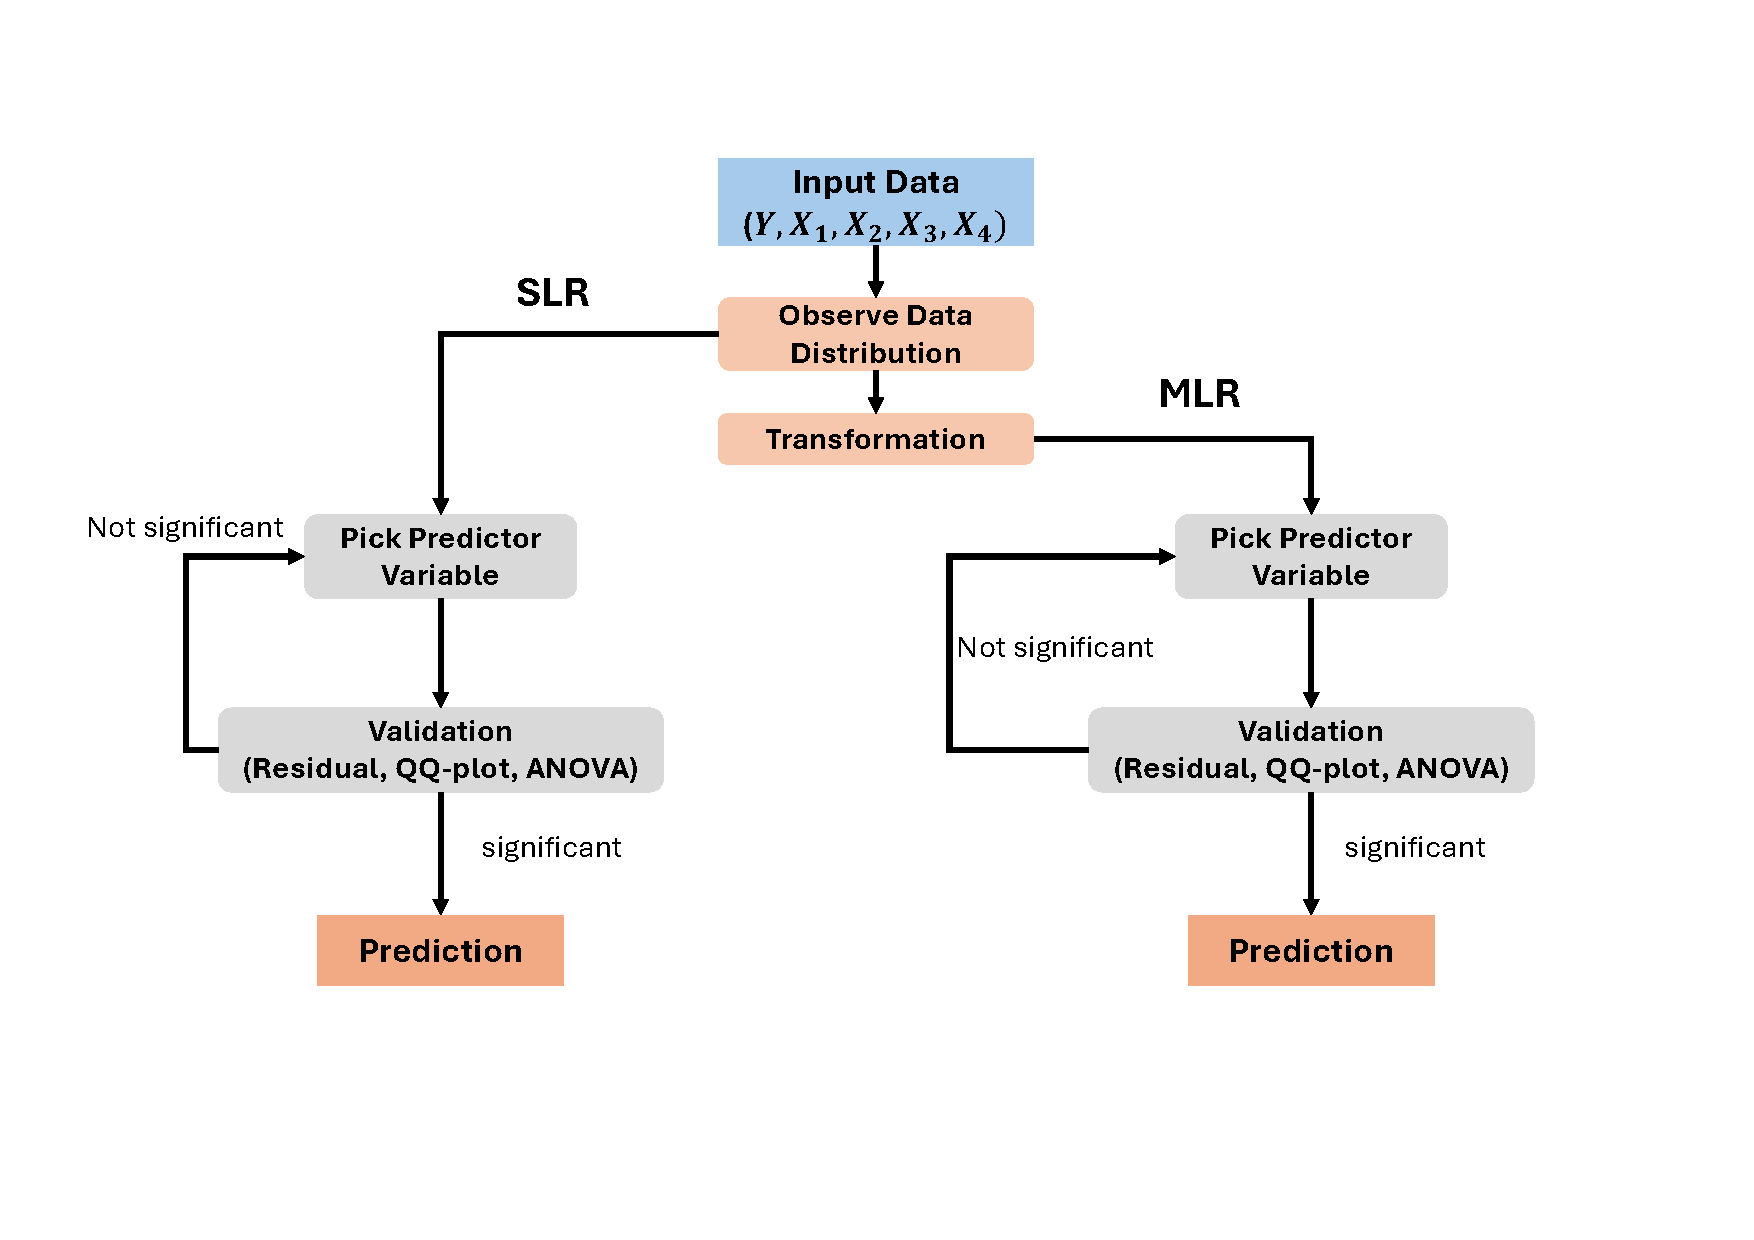
\includegraphics[width=1\linewidth]{figures/Intro.pdf}
    \caption{An overview of our pipeline.}
    \label{fig:intro}
\end{figure}

% 这部分就画画流程图,大概讲一下我们的流程
% 主要大概就是 overview -> slr -> mlr